%%% Thesis Introduction --------------------------------------------------
\chapter{Introduction}\label{ch:Introduction}
\ifpdf
    \graphicspath{{Introduction/IntroductionFigs/PNG/}{Introduction/IntroductionFigs/PDF/}{Introduction/IntroductionFigs/}}
\else
    \graphicspath{{Introduction/IntroductionFigs/EPS/}{Introduction/IntroductionFigs/}}
\fi

\section{Problem overview}
Transient pulses in an audio stream originating from the physical interaction with a device, are a common feature of modern integrated devices. Microphones are typically incorporated into laptop computers, mobile phones and tablets due to their low price and relatively high utility in relation to single or multi-channel audio recordings or for noise or echo-cancellation applications. The primary function of the embedded microphones is typically to pick up external sounds (external to the device), but as a consequence of the mechanical construction, microphones tend to pick up physical interactions with the device as well. In devices with embedded keyboards, typing will often produce clearly audible transient pulses in the audio stream, e.g. a conference call, which may be considered a nuisance and even cause a loss of intelligibility. Even interactions via non-physical keys, e.g. touchscreens, will produce a clearly audible pulse in the audio stream of a device. While these audible pulses would be considered a nuisance in the context of a conference call, it is possible that they could provide additional information about the origin of touch interactions in others.

\section{Aims and objectives}
The work presented here will consider two aspects of impact related audio pulses. Firstly the pulses will be considered from a functional perspective as a means for localising impacts, and secondly the pulses will be considered as an annoyance or deleterious effect in the form of noise. It is noted that these two perspectives are not necessarily mutually exclusive, i.e. one might wish to both classify and then remove such a transient.

\subsection{Acoustic pulse recognition (APR)}
\emph{Is it possible to accurately infer the origin of a device-interaction solely based on the audible pulse generated from the interaction?}
This question will be considered primarily from the perspective of a single-channel input and will focus on methods that are computationally realisable in a real-time scenario. The problem will be framed as a touchscreen implementation and will be referred to as \gls{apr}. The performance of the methods developed will be compared and contrasted and various practical concerns associated with the particular application will be discussed. An extension of the application will seek to generalise the application to multiple channels.

An example of a pulse associated with the interaction with a device is shown in Figure~\ref{fig:singleSampleTap.png}. This pulse is recorded from a standard mobile phone (more details in section~\ref{sec:APRsystem}), and the majority of the pulse has decayed after approximately 7 ms.

\begin{figure}
  \begin{center}
    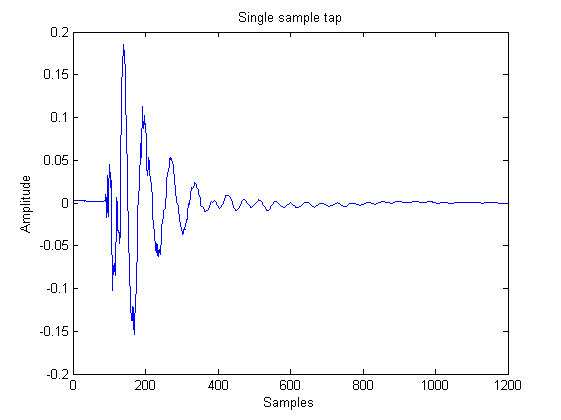
\includegraphics[width=110mm]{singleSampleTap.png}
    \caption{A sample pulse from a mobile phone. Sampled at 44.1 kHz.}\label{fig:singleSampleTap.png}
  \end{center}
\end{figure}

A successful application of a classification algorithm relies on the similarity of pulses from identical impact sites and dissimilarity from those from other sites. Figure~\ref{fig:twotwoSampleTap.png} shows an example of four pulses: two from one spot (blue) and two from a different spot (red). It is clearly seen in Figure~\ref{fig:twotwoSampleTap.png} that while the blue pulses are nearly identical their waveforms are vastly different to that of the red pulses. This observation is, as noted, integral to a successful classification algorithm based on this data. In this example all pulse-onsets have been aligned to the same point.

\begin{figure}
  \begin{center}
    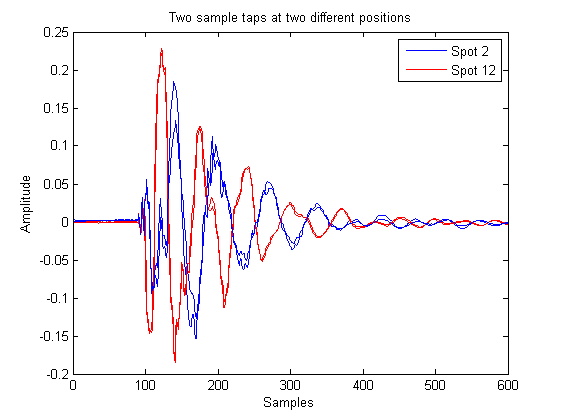
\includegraphics[width=110mm]{twotwoSampleTap.png}
    \caption{Two sets of two sample pulses recorded a two different spots on the mobile phone. Sampled at 44.1 kHz.}\label{fig:twotwoSampleTap.png}
  \end{center}
\end{figure}

While Figure~\ref{fig:twotwoSampleTap.png} shows data obtained in an ideal scenario, pulses will vary greatly depending on factors such as temperature, how the device is suspended and with what it is impacted. The work undertaken in chapters~\ref{ch:APR} and~\ref{ch:MultichannelAPR} will seek to apply this classification algorithm as a real world touch surface application.

% Summary of literature
%A range of applications have been proposed that utilise multiple microphones to implement a touchscreen interface \cite{US8174547}\cite{US8233353}\cite{TouchSystems2006}\cite{US7411581}\cite{WO2006108443}. The functional elements of these methods all rely on their being multiple sources and so the single-channel implementation of the \gls{apr} system is radically different and should therefore be considered a significant contribution. Not only does the single-channel implementation of the \gls{apr} system allow for lower hardware cost for integration, it also enables post-hoc integration in system without multiple accessible microphones which currently still is the majority of devices. Work presented in chapter~\ref{ch:APR} is also presented in \cite{Christensen2011} and \cite{US20110316784}.

\subsection{Keyboard stroke removal}
\emph{Is it possible to remove or reduce the effect of transient noise pulses, in particular keyboard stroke noise, on a real-time single channel audio stream for teleconferencing applications?}
This question will again be considered in the context of a realistic teleconferencing scenario. The implementation will be limited by the practical constraints of the webRTC platform and feature a sampling frequency of 16 kHz and buffers of 256 samples with 96 samples of overlap between buffers, leaving 10 ms of new data per buffer. In addition, the system needs to be applicable in a real-time scenario, setting limits to the computational requirements of the system. The system should be unsupervised, require no training, work on, and remove, a multitude of noise pulses while letting speech signals through unaffected. The system being developed can roughly be divided into two separate parts: a detection stage and a restoration stage. It is the aim to detect pulses reliably while embedded in speech segments, accurately in time and with as few false detections as possible. Restorations of the detected pulses should aim to decrease the nuisance associated with the noise pulses and restored and interpolated segments should be unobtrusive and preferably unnoticeable.

The primary focus of this noise removal algorithm concern the noise pulses associated with keyboard typing strokes. As with the more general pulses associated with the classification application, the keyboard stroke pulses vary greatly with a range of factors but more importantly they vary between devices. This is a particular issue given that the algorithm specifications requires the algorithm to be unsupervised and will therefore not able to learn the particular signature of keystrokes on a particular device.

Figure~\ref{fig:KeyboardStrokeSlowIntro.pdf} shows an example of the waveform from a single slowly typed keystroke. This single keyboard stroke is noticeably comprised of two individual pulses, where the initial sharply rising pulse is associated with the physical action of the mechanical key being pressed and the secondary lower amplitude pulse nearly 200 ms after the initial pulse is associated with the lifting of the finger from the button. This delay between the two pulses is what defines this keyboard stroke as \emph{slow}, whereas faster typing can leave gaps much shorter. It is also noted that there is a significant slowly decaying low frequency component associated with each individual pulse.

\begin{figure}
  \begin{center}
    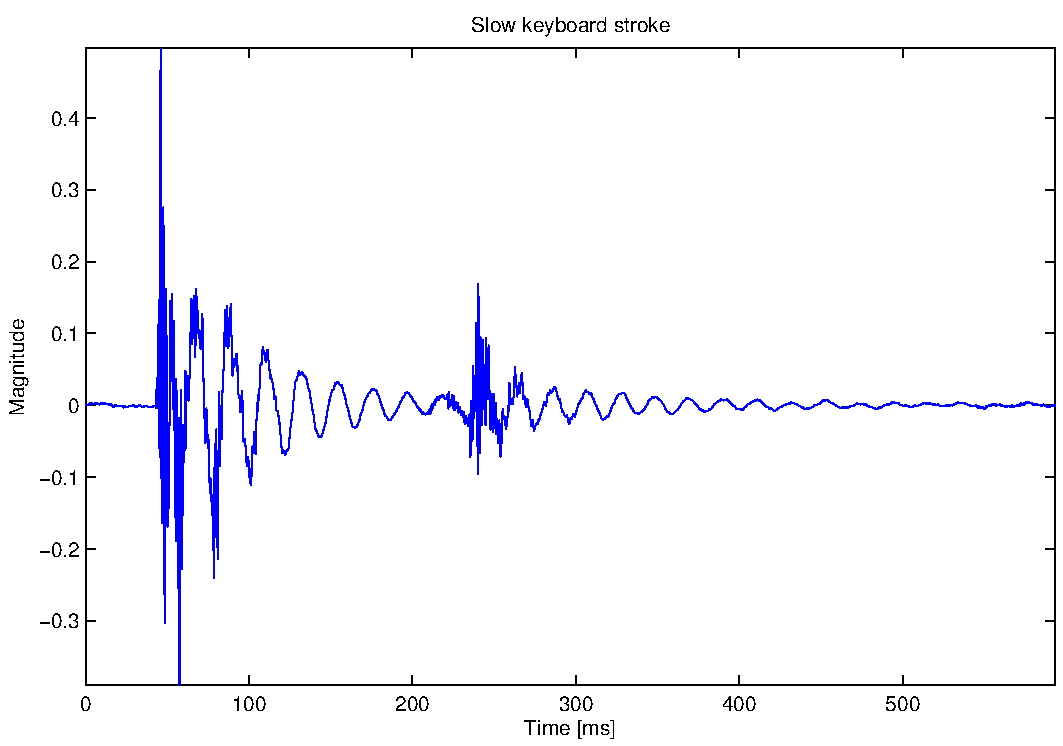
\includegraphics[width=110mm]{KeyboardStrokeSlowIntro.pdf}
    \caption{A sample keystroke sampled at 44.1 kHz.}\label{fig:KeyboardStrokeSlowIntro.pdf}
  \end{center}
\end{figure}

Figure~\ref{fig:shortFastSeq.png} shows the keyboard strokes in the context of a short rapidly typed 5 stroke sequence. The lift-pulses can be seen to appear right before (approximately 10 ms) the second, third and fourth stroke whereas the rest of the lift-pulses are more delayed. It is also noted that while these four primary keystroke-pulses are part of the same sequence they are visually dissimilar. It is also noted that the first stroke clearly shows two distinct pulses in the waveform while an audible evaluation only reveals a single pulse. It is clear that pulses arising from real life typing are extremely varied with only a few common features, one of which is an initial clear sudden rise noted in the signal amplitude.

\begin{figure}
  \begin{center}
    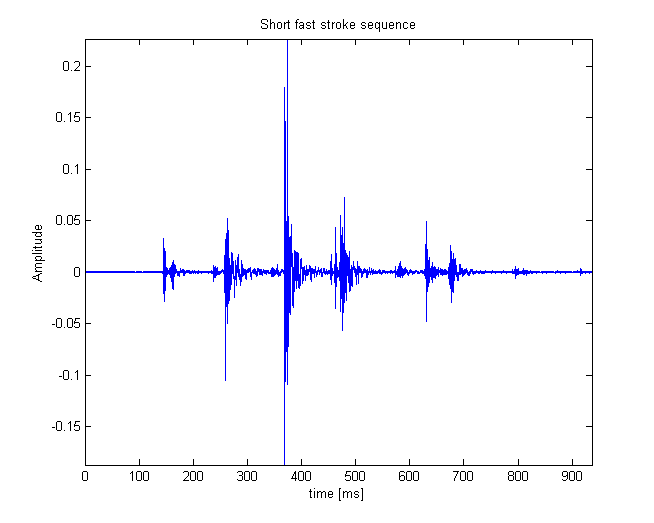
\includegraphics[width=110mm]{shortFastSeq.png}
    \caption{A quickly typed sequence of 5 keyboard strokes sampled at 44.1 kHz.}\label{fig:shortFastSeq.png}
  \end{center}
\end{figure}

Figure~\ref{fig:shortFastSeqSpec.png} shows a spectrogram of the typing sequence displayed in Figure~\ref{fig:shortFastSeq.png}. It is noted that all pulses exhibit a short sudden burst of energy across the spectrum. Even the lift-pulses exhibit this characteristic at a lower level. With each pulse is also a clearly identifiable burst of low frequency energy, in the range of human speech, which clearly outlasts the higher frequency components in time.

\begin{figure}
  \begin{center}
    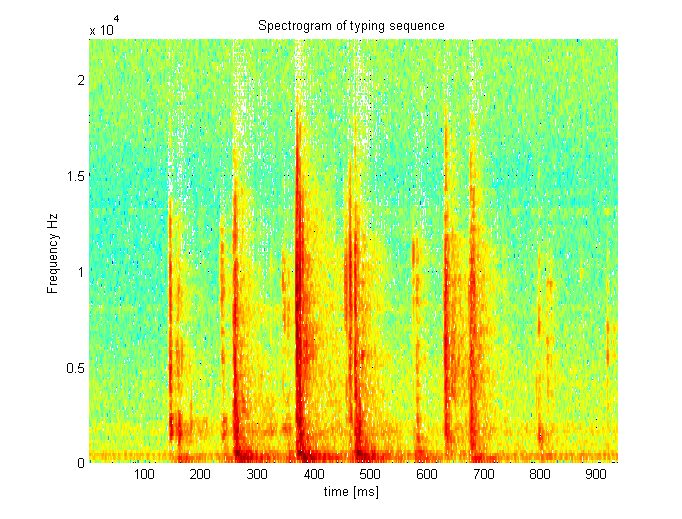
\includegraphics[width=110mm]{shortFastSeqSpec.png}
    \caption{Spectrogram of the same sequence of 5 keystrokes as in Figure~\ref{fig:shortFastSeq.png}. Sampled at 44.1 kHz.}\label{fig:shortFastSeqSpec.png}
  \end{center}
\end{figure}

A thorough investigation of the data associated with this application will be conducted in section~\ref{sec:WPdata}, but with this initial investigation the distinguishing features of interest in keyboard typing pulses are a wide spectral response and rapid onset with lingering low frequency components. The temporal extent of the initial pulses typically range from 30 ms to over 300 ms.

%in the literature (summary)
%A couple of articles have suggested similar systems \cite{Subramanya2007}\cite{Sugiyama2007}\cite{Abramson2007}. \cite{Subramanya2007} and \cite{Sugiyama2007} propose algorithms specifically for the keyboard stroke detection and removal application. All of these methods rely on \gls{stft} as a basis for detection using features such as the shape of and change of the power spectrum \cite{Sugiyama2007}, \gls{ar} estimation error \cite{Subramanya2007}\cite{Kauppinen2002} or a Bayesian speech estimator \cite{Abramson2007}. In \cite{Godsill1998book} various \gls{ar} based detection methods are proposed and it was found that pairing the \gls{ar} model with a basis, e.g. a sinusoid, gives a generally applicable approach with improved performance. In \cite{Vaseghi1990} the authors find that \gls{ar} processes are ``adequate for modelling of speech signals whereas they can not model impulsive disturbances.''.
%
%Restoration approaches applicable to longer gaps ranged from heuristic waveform substitution methods \cite{Goodman1986}\cite{Niediwiecki2001}, pitch based methods modeling speech as spectral peak tracks \cite{Maher1994}\cite{McAulay1986} to \gls{ar} interpolators \cite{Esquef2006} based on a least squares adaption of the \gls{ar} process \cite{Godsill1998book}.
%synthesis filters designed to excite the \gls{ar} model to achieve longer gap extrapolation with lower model orders \cite{Esquef2006}

%\section{Scope of the thesis and contributions to knowledge}

\section{Terminology}
%pulse/impulse
%noise
%Transient noise used when focus on noise.
Throughout the literature the terms \emph{pulse}\cite{Esquef2002a}\cite{Esquef2003a} and \emph{impulse}\cite{Czyzewski1995}\cite{Kauppinen2002a}\cite{Chen2000} have been used interchangeably to refer to a short burst of sound. Generally the use of the term \emph{click}\cite{Czyzewski1995}\cite{Esquef2002}\cite{Godsill1998book} has been associated with physical defects in a recording medium or other extremely short term corruptions. Henceforth the term \emph{pulse} will be used to describe the specific audio signals of interest throughout this work, for its alignment with the already established term \gls{apr}\cite{TouchSystems2006}. The term \emph{noise}, or the more specific \emph{impulsive noise} and \emph{transient noise}, will only be used to refer to specifically unwanted aspects of the signal and will as such mainly be used in chapters~\ref{ch:TransientNoiseDetection} and \ref{ch:TransientNoiseRestoration}.

%Keyboard stroke pulse (sometimes pulse sequence) vs. single pulse
In chapters~\ref{ch:TransientNoiseDetection} and \ref{ch:TransientNoiseRestoration} the term \emph{keyboard stroke} or \emph{key stroke} will be used to specifically refer to the sequence of disturbances that arise from the typing action on a keyboard. These sequences will in many cases encompass a series of \emph{pulses}.

%Chapter~\ref{ch:TransientNoiseRestoration} is commonly referred to as the \emph{restoration} chapter, but the term \emph{reconstruction} has also in some places been applied somewhat interchangeably. In general the term \emph{restore} has been used more generally as any action that aims to alleviate \emph{defects}, \emph{artifacts} or \emph{noise}. \emph{Reconstruct} refers more specifically to situations where samples are discarded and replaced with new estimates. An example of a \emph{restoration} that would not be a \emph{reconstruction} is a scaling action of corrupted samples. In the same chapter the terms \emph{interpolation} and \emph{extrapolation} has been used in some contexts interchangeably. In general \emph{interpolate} is used to refer to action where samples are inserted in between other samples by some means, e.g. linear interpolation, where \emph{extrapolate} refers to the extension of a signal with no pre-defined end points, e.g. prediction. Typically \emph{interpolation} is here more often used to refer to the non-real-time applications that in most cases end up being \emph{extrapolation} when applied in real-time due to the general rule of causality.

\section{About this thesis}
This thesis is structured as follows; Following this introductory chapter the literature review is presented in chapter~\ref{ch:LiteratureReview}. Here the surveyed literature is presented in sections relevant to their occurrence in the thesis. Chapter~\ref{ch:APR} introduces the pulse classification or \gls{apr} system and the main theory. Results are also presented outlining detection performance and the model's sensitivity to certain parameters. Chapter~\ref{ch:MultichannelAPR} presents a multi-channel generalisation of the basic model derived in chapter~\ref{ch:APR}. Results are presented, in chapter~\ref{ch:MultichannelAPR}, from extensive testing in clean and noisy environments. Chapters~\ref{ch:TransientNoiseDetection} and~\ref{ch:TransientNoiseRestoration} should be considered together as the transient noise suppression system, where chapter~\ref{ch:TransientNoiseDetection} presents methods for the detection of pulses including a proposed pre-processing stage and chapter~\ref{ch:TransientNoiseRestoration} builds on the previous work and considers a number of restoration approaches for the detected pulses. The thesis ends with the conclusions in chapter~\ref{ch:Conclusions}. Here the aims for the work presented in the introduction are reevaluated in the context of the work undertaken. The major contributions are restated and a summary of the proposed future work is presented.

Work presented in chapter~\ref{ch:APR} is also presented in \cite{Christensen2011} and \cite{US20110316784}.
%%% ----------------------------------------------------------------------


%%% Local Variables:
%%% mode: latex
%%% TeX-master: "../thesis"
%%% End:
